\documentclass{article}
\usepackage[utf8]{inputenc}
\usepackage{hyperref}
\usepackage[letterpaper, portrait, margin=1in]{geometry}
\usepackage{enumitem}
\usepackage{amsmath}
\usepackage{booktabs}
\usepackage{graphicx}

\usepackage{hyperref}
\hypersetup{
colorlinks=true,
    linkcolor=black,
    filecolor=black,      
    urlcolor=blue,
    citecolor=black,
}
\usepackage{natbib}

\usepackage{titlesec}
  
\title{Homework 2 }
\author{Economics 7103}
\date{Spring semester 2023}
  
\begin{document}
  
\maketitle


Q1) The randomization seems to have worked and difference in mean seems to be unbiased.
\begin{table}[ht]
    \centering
    \begin{tabular}{llll}
\toprule
{} &   Control & \multicolumn{2}{l}{Treatment} \\
{} &      Mean &      Mean & p-value \\
{} & (Std dev) & \multicolumn{2}{l}{(Std dev)} \\
\midrule
electricity &   1181.33 &   1086.75 &    0.00 \\
            &    454.31 &    423.96 &         \\
sqft        &   1633.05 &   1657.55 &    0.57 \\
            &    682.90 &    686.27 &         \\
temp        &     79.89 &     79.89 &    0.99 \\
            &      2.16 &      1.97 &         \\
\bottomrule
\end{tabular}

    \caption{Q1 Diff of Means- Python}
    \label{tab:mean_py}
\end{table}


Q2
Graph:
\begin{figure}[h]
    \centering
    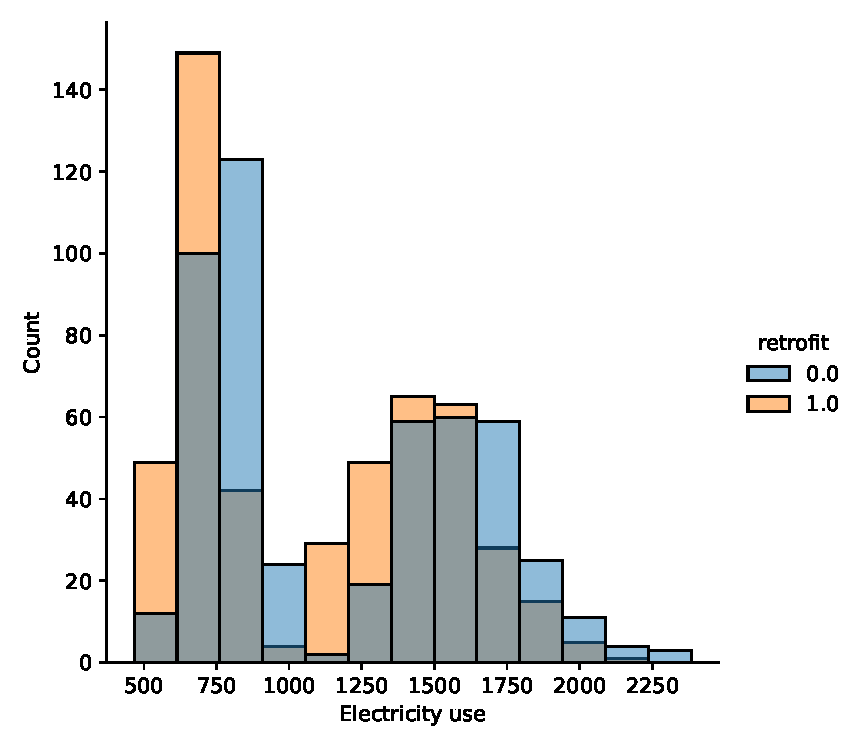
\includegraphics[width=50mm]{Q2_hist.pdf}
    \caption{Histogram}
    \label{fig:hist_py}
\end{figure}


\begin{table}[ht!]
Q3
A.
    \centering
    \begin{tabular}{lr}
\toprule
{} &   Estimates \\
\midrule
Constant &  -83.602758 \\
sqft     &    0.615339 \\
temp     &    3.255075 \\
retrofit & -109.666176 \\
\bottomrule
\end{tabular}

    \caption{Q3.a) OLS by hand - Python}
    \label{tab:ols_hand}
\end{table}


\begin{table}[ht!]
Q3
B.
    \centering
    \begin{tabular}{lr}
\toprule
{} &   Estimates \\
\midrule
Constant &  -83.557159 \\
sqft     &    0.615338 \\
temp     &    3.254511 \\
retrofit & -109.666472 \\
\bottomrule
\end{tabular}

    \caption{Q3.b) OLS using SLS}
    \label{tab:ols_sls}
\end{table}

\begin{table}[h!]
Q3
C.  \centering
    \begin{tabular}{ll}
\toprule
{} &       Estimates \\
\midrule
Variable 1   &           -3.25 \\
             &   (-3.9, -2.64) \\
Variable 2   &           12.55 \\
             &  (12.11, 13.02) \\
Constant     &           -14.0 \\
             &   (-23.3, -6.0) \\
Observations &             100 \\
\bottomrule
\end{tabular}

    \caption{Q3.c)OLS produced using Python - Statsmodel}
    \label{tab:olssm}
\end{table}



\begin{figure}[h!]
Q4
Diff of Means Table - Stata:

    \centering
    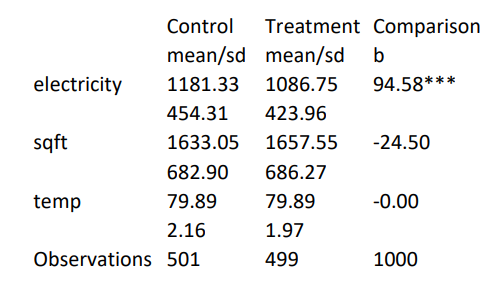
\includegraphics[width=70mm]{means_stata.png}
    \caption{Difference of Means}
    \label{fig:means_stata}
\end{figure}


\begin{figure}[h!]
Q5
Two-way Scatter Plot:

    \centering
    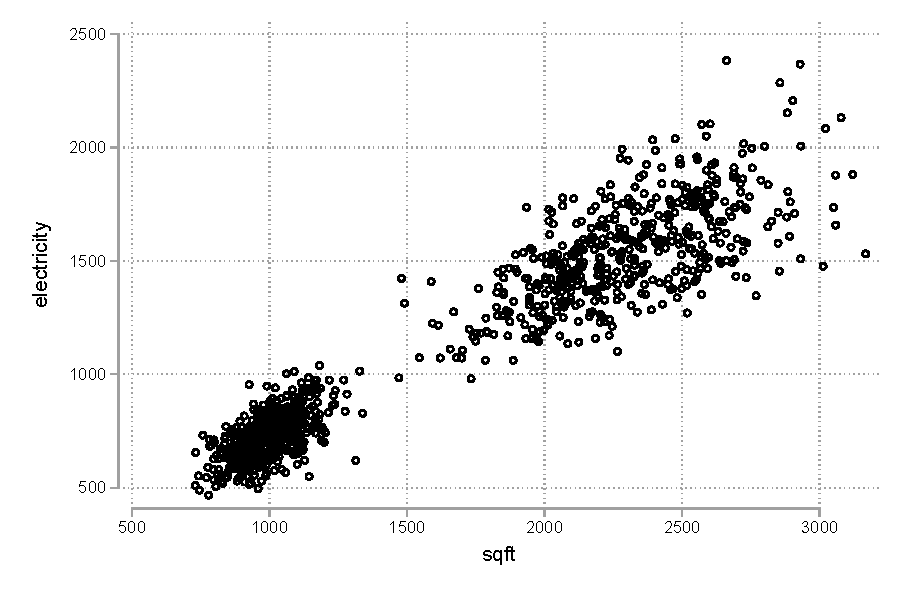
\includegraphics[width=80mm]{twoway_stata.pdf}
    \caption{Two way plot}
    \label{fig:graph_stata}
\end{figure}




\begin{table}[h!]
Q6
    \centering
    \begin{tabular}{lc} \hline
 & (1) \\
VARIABLES & Ordinary least squares \\ \hline
 &  \\
sqft & 0.62** \\
 & (0.01) \\
temp & 3.26 \\
 & (1.92) \\
retrofit & -109.67** \\
 & (7.95) \\
Constant & -83.60 \\
 & (154.36) \\
 &  \\
Observations & 1,000 \\
 R-squared & 0.92 \\ \hline
\multicolumn{2}{c}{ Standard errors in parentheses} \\
\multicolumn{2}{c}{ ** p$<$0.01, * p$<$0.05} \\
\end{tabular}

    \caption{OLS produced using Stata}
    \label{tab:statasummary}
\end{table}



\end{document}